%
% exemplo genérico de uso da classe iiufrgs.cls
% $Id: iiufrgs.tex,v 1.1.1.1 2005/01/18 23:54:42 avila Exp $
%
% This is an example file and is hereby explicitly put in the
% public domain.
%
\documentclass[cic,tc]{iiufrgs}
\usepackage{tikz}
\usepackage{tikz-3dplot}
\usetikzlibrary{calc,arrows.meta,positioning,backgrounds}
\usepackage{gensymb}
\tdplotsetmaincoords{-60}{-35}

% Para usar o modelo, deve-se informar o programa e o tipo de documento.
% Programas :
% * cic       -- Graduação em Ciência da Computação
% * ecp       -- Graduação em Ciência da Computação
% * ppgc      -- Programa de Pós Graduação em Computação
% * pgmigro   -- Programa de Pós Graduação em Microeletrônica
%
% Tipos de Documento:
% * tc                -- Trabalhos de Conclusão (apenas cic e ecp)
% * diss ou mestrado  -- Dissertações de Mestrado (ppgc e pgmicro)
% * tese ou doutorado -- Teses de Doutorado (ppgc e pgmicro)
% * ti                -- Trabalho Individual (ppgc e pgmicro)
%
% Outras Opções:
% * english    -- para textos em inglês
% * openright  -- Força início de capítulos em páginas ímpares (padrão da
% biblioteca)
% * oneside    -- Desliga frente-e-verso
% * nominatalocal -- Lê os dados da nominata do arquivo nominatalocal.def


% Use unicode
\usepackage[utf8]{inputenc}   % pacote para acentuação

% Necessário para incluir figuras
\usepackage{graphicx}         % pacote para importar figuras

\usepackage{times}            % pacote para usar fonte Adobe Times
% \usepackage{palatino}
% \usepackage{mathptmx}       % p/ usar fonte Adobe Times nas fórmulas

\usepackage[alf,abnt-emphasize=bf]{abntex2cite}	% pacote para usar citações abnt

%
% Informações gerais
%
\title{Estimativa de profundidade a partir de uma única imagem omnidirecional}

\author{Dal'Aqua}{Lorenzo Pezzi}

% orientador e co-orientador são opcionais (não diga isso pra eles :))
\advisor[Prof.~Dr.]{Jung}{Claudio}
% \coadvisor[Prof.~Dr.]{Knuth}{Donald Ervin}

% a data deve ser a da defesa; se nao especificada, são gerados
% mes e ano correntes
\date{11 de Janeiro}{2018}

% o local de realização do trabalho pode ser especificado (ex. para TCs)
% com o comando \location:
% \location{Itaquaquecetuba}{SP}

% itens individuais da nominata podem ser redefinidos com os comandos
% abaixo:
% \renewcommand{\nominataReit}{Prof\textsuperscript{a}.~Wrana Maria Panizzi}
% \renewcommand{\nominataReitname}{Reitora}
% \renewcommand{\nominataPRE}{Prof.~Jos{\'e} Carlos Ferraz Hennemann}
% \renewcommand{\nominataPREname}{Pr{\'o}-Reitor de Ensino}
% \renewcommand{\nominataPRAPG}{Prof\textsuperscript{a}.~Joc{\'e}lia Grazia}
% \renewcommand{\nominataPRAPGname}{Pr{\'o}-Reitora Adjunta de P{\'o}s-Gradua{\c{c}}{\~a}o}
% \renewcommand{\nominataDir}{Prof.~Philippe Olivier Alexandre Navaux}
% \renewcommand{\nominataDirname}{Diretor do Instituto de Inform{\'a}tica}
% \renewcommand{\nominataCoord}{Prof.~Carlos Alberto Heuser}
% \renewcommand{\nominataCoordname}{Coordenador do PPGC}
% \renewcommand{\nominataBibchefe}{Beatriz Regina Bastos Haro}
% \renewcommand{\nominataBibchefename}{Bibliotec{\'a}ria-chefe do Instituto de Inform{\'a}tica}
% \renewcommand{\nominataChefeINA}{Prof.~Jos{\'e} Valdeni de Lima}
% \renewcommand{\nominataChefeINAname}{Chefe do \deptINA}
% \renewcommand{\nominataChefeINT}{Prof.~Leila Ribeiro}
% \renewcommand{\nominataChefeINTname}{Chefe do \deptINT}

% A seguir são apresentados comandos específicos para alguns
% tipos de documentos.

% Trabalho Individual [ti]:
% \ti{123}     % numero do TI
% \ti[II]{456} % no caso de ser o segundo TI

%
% palavras-chave
% iniciar todas com letras minúsculas, exceto no caso de abreviaturas
%
\keyword{imagens omnidirecionais}
\keyword{estimativa de profundidade}
\keyword{CNNs}
\keyword{equiretangular}

%\settowidth{\seclen}{1.10~}

%
% inicio do documento
%
\begin{document}

% folha de rosto
% às vezes é necessário redefinir algum comando logo antes de produzir
% a folha de rosto:
% \renewcommand{\coordname}{Coordenadora do Curso}
\maketitle

% dedicatoria
% \clearpage
% \begin{flushright}
%     \mbox{}\vfill
%     {\sffamily\itshape
%       ``If I have seen farther than others,\\
%       it is because I stood on the shoulders of giants.''\\}
%     --- \textsc{Sir~Isaac Newton}
% \end{flushright}

% agradecimentos
%\chapter*{Agradecimentos}
%Agradecimentos...



% resumo na língua do documento
\begin{abstract}
    Abstract em português
\end{abstract}

% resumo na outra língua
% como parametros devem ser passados o titulo e as palavras-chave
% na outra língua, separadas por vírgulas
\begin{englishabstract}{Depth estimation on a single omnidirectional image}{Keywords, in, English}
    Abstract in english
\end{englishabstract}

% lista de figuras
\listoffigures

% lista de tabelas
\listoftables

% lista de abreviaturas e siglas
% o parametro deve ser a abreviatura mais longa
\begin{listofabbrv}{ABREV}
    \item[ABREV] Abreviatura
    \item[SIG] Sigla
\end{listofabbrv}

% idem para a lista de símbolos
\begin{listofsymbols}{$\alpha\beta\pi\omega$}
    \item[$\sum{\frac{a}{b}}$] Somatório do produtório
    \item[$\alpha\beta\pi\omega$] Fator de inconstância do resultado
\end{listofsymbols}

% sumario
\tableofcontents

% aqui comeca o texto propriamente dito

% introducao
\chapter{Introdução}

Este trabalho introduz um método para a estimativa de profundidade a partir de uma única imagem omnidirecional. Iniciaremos introduzindo os conceitos básicos sobre imagens omnidirecionais e estimativa de profundidade.

\section{Imagens perspectivas e imagens omnidirecionais}

As áreas de visão computacional e processamento de imagens, comumente trabalham com imagens planares, onde a luz de uma cena em três dimensões é projetada para um plano de duas dimensões através da projeção perspectiva. Imagens planares são capturadas através de câmeras, que tem um funcionamento parecido com o olho humano, e possuem um campo de visão limitado, normalmente em até 180\degree, e quanto maior o campo de visão mais distorcidas são as imagens. A projeção perspectiva projeta pontos do espaço \textit{3D} para um plano \textit{2D}, no caso de imagens digitais, em pontos discretos.

\begin{figure}
    \caption{Projeção perspectiva}
    \begin{center}
    \resizebox {15em} {!} {
	\begin{tikzpicture}
  [
    tdplot_main_coords,
    >=Stealth,
    my dashed/.style={dashed, thick, ->, shorten >=-15pt, shorten <=-15pt, every node/.append style={font=\footnotesize}},
    my box/.style={thin, gray!70},
    my blue/.style={blue, line cap=round, -{Triangle[width=3*#1]}, line width=#1, shorten >=#1*1.75pt, every node/.append style={fill, circle, inner sep=0pt, minimum size=#1*3.5pt, anchor=center, outer sep=0pt}},
    my label/.append style={midway, font=\scriptsize},
    my vectors/.style={green!50!black, {Stealth[scale=.75]}-{Stealth[scale=.75]}},
    my red/.style={thick, red, line cap=round},
    my grey/.style={gray!70},
    description/.style={draw=gray!70, thick, line cap=round, every node/.style={align=center, font=\scriptsize\sffamily, anchor=north}},
  ]
%   \draw [help lines] (-2,0,0) -- (2,0,0) node[anchor=north west]{$x$} (0,0,0) -- (0,7,0) node[anchor=north east]{$y$} (0,0,0) -- (0,0,2) node[anchor=north]{$z$} (-2,7,0) -- (2,7,0);
  \draw [my grey] (0,4,0) -- (0,7,0) (-2,7,0) -- (2,7,0);
  \coordinate (o) at (0,0,0);
  \path [draw=gray!70, text=gray, fill=gray!20, opacity=0.8, text opacity=1] (-1.5,4,1.75) coordinate (a) -- ++(0,0,-3.5) coordinate (b) -- ++(3,0,0) coordinate (c) -- ++(0,0,3.5) coordinate (d) -- cycle node [pos=.95, above, sloped, anchor=south west] {$z=f$} ;
%   \foreach \i in {a,b,c,d} \node [red, font=\scriptsize] at (\i) {\i};
  \draw [my grey] (-2,0,0) -- (2,0,0) (0,0,0) -- (0,4,0) (0,0,0) -- (0,0,2);
  \draw [thick, ->, every node/.style={font=\footnotesize, inner sep=0pt}] (o) node [anchor=north west] {$F_c$} (o) edge node [pos=1, anchor=north east] {$z_c$} ++(0,1,0) edge node [pos=1, anchor=north] {$y_c$} ++(0,0,1) -- ++(1,0,0) node [anchor=north west] {$x_c$};
  \draw [my box] (o) ++(0,4,-.5) coordinate (p1) -- ++(1,0,0) coordinate (p2) -- ++(0,0,-1.25) coordinate (p3);
  \foreach \i in {0,1,...,4} \draw [my box] (p1) ++(\i*.25,0,0) -- ++(0,0,-.25);
  \foreach \i in {0,1,...,5} \draw [my box] (p2) ++(0,0,-\i*.25) -- ++(-.25,0,0);
  \draw [my box] (p1) ++(0,0,-.25) -- ++(.75,0,0) -- ++(0,0,-1);
  \draw [my dashed, cyan] ($(b)!1/2!(c)$) -- ($(d)!1/2!(a)$) node [below=15pt, anchor=north] {$y$};
  \draw [my dashed, cyan] ($(b)!1/2!(a)$) -- ($(d)!1/2!(c)$) node [above right=17pt, anchor=north west] {$x$};
  \draw [my dashed, green!50!black, <->] (a) node [below=15pt, anchor=north] {$v$} -- (b) -- (c) node [above right=17pt, anchor=north west] {$u$};
  \path [green!50!black, every node/.style={font=\scriptsize, inner sep=0pt}] (p2) node [above right, anchor=south west] {$(u,v)$};
  \path (p2) ++(-.125,0,0) coordinate (q2) ++(0,0,-.125) coordinate (r2);
  \draw [my blue=1] ($(0,4,0)+($(q2)-(p1)$)$) coordinate (s2) -- (r2) node (d1) {};
  \scoped[on background layer]{\draw [my blue=1.75] ($($1.75*($(s2)-(0,4,0)$)$)+(0,7,0)$) -- ++($1.75*($(r2)-(s2)$)$) node (d2) [label={[label distance=-20pt]above:{$P=(X,Y,Z)$}}] {};}
  \draw [my vectors] (0,4,.1) -- ($(s2)+(0,0,.1)$) node [below, my label, sloped] {$\vec{u}$};
  \draw [my vectors] (-.1,4,0) -- ($(q2)-(s2)+(-.1,4,0)$) node [left, my label] {$\vec{v}$};
  \draw [my red] (o) -- (d1.center);
  \scoped[on background layer]{\draw [my red] (d1.center) -- (d2.center);}
  \path [description] (0,4,0) [out=-95, in=95] to (-.75,4,.25) node {ponto\\principal} (0,6.5,0) [out=-95, in=95] to (-.75,6.5,.25) node {eixo\\\'otico};
		\end{tikzpicture}
	}
    \end{center}
    \label{fig:perspectiveProj}
    \legend{Fonte: https://tex.stackexchange.com/q/96074/}
\end{figure}

Imagens omnidirecionais, também conhecidas como imagens esféricas, capturam a luz de todas as direções ao redor do ponto onde são capturadas, possuindo um campo de visão de 360\degree, logo as distorções que seriam introduzidas com a projeção perspectiva são muito mais significativas. Para trabalhar com imagens esféricas são utilizadas diferentes projeções para mapear a esfera de três dimensões para uma imagem em duas dimensões. Há as projeções cilíndricas, azimutais, entre outras (citar panotools wiki), e ao longo do trabalho será utilizada a projeção equiretangular somente. Nesta projeção,  como descrito na figura \ref{fig:sphericalIm}, os 360\degree do campo de visão horizontal são projetados em W pixels e os 180\degree de campo de visão vertical em H pixels.

\begin{figure}
    \caption{Imagem omnidirecional em projeção equiretangular}
    \begin{center}
        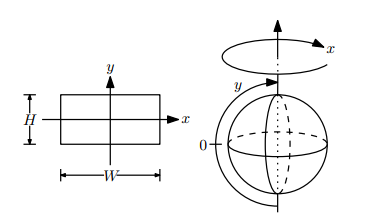
\includegraphics[width=20em]{equiretangular.png}
    \end{center}
    \label{fig:sphericalIm}
    \legend{Fonte: Jianxiong Xiao, 3D Geometry for panorama}
\end{figure}

\section{Estimativa de profundidade}

A estimativa de profundidade consiste em, através da informação de cor de uma ou mais imagens, estimar a profundidade de cada pixel no espaço tridimensional. Há múltiplas aplicações em robótica, como navegação e reconhecimento de objetos, além de ser um componente essencial para a reconstrução 3D. No caso de imagens esféricas, a reconstrução 3D de uma imagen 360\degree tem aplicações diretas em realidade virtual e realidade aumentada.

O método clássico para estimativa de profundidade é o \textit{stereo matching}, onde a partir de um par de imagens, a profundidade é estimada utilizando a correspondência entre pixels das duas imagens. Para tanto, é preciso utilizar câmeras cujos parâmetros sejam conhecidos. Recentemente, a aplicação de redes neurais convolucionais mostrou resultados impressionantes na estimativa de profundidade a partir de uma única imagem. No entanto, a utilização destes algoritmos com imagens 360\degree não produz a mesma qualidade de resultados, pois o treinamento destes é feito utilizando imagens perspectivas.

O método proposto neste trabalho pretende estender as técnicas de estimação de profundidade a partir de uma única imagem perspectiva para o domínio das imagens esféricas. Para tanto, são feitas projeções planares de seções da imagem esférica, e é estimada a profundidade de cada seção. As profundidades calculadas são projetadas de volta para o domínio esférico, porém as profundidades estimadas para cada seção não são coerentes entre si. Para gerar uma mapa de profundidades suave são escolhidas seções com regiões sobrepostas, então é feita uma minimização da diferença das profundidades nas regiões sobrepostas através da ponderação da profundidade de cada seção na imagem final.

% Comentar sobre resultados aqui...


\chapter{Trabalhos anteriores}

\section{Imagens omnidirecionais}
Sun360

\section{Stereo matching em imagens omnidirecionais}
Stereo matching pode ser usado para imagens omnidirecionais, já usam em colagens (citar \citep{Li2001})

\section{Estimativa de profundidade a partir de uma única imagem}
Técnicas de estimativa de profundidade a partir de uma única imagem já eram pesquisadas desde os anos 90 (citar), mas a partir do uso de redes neurais que os resultados ficaram interessantes

\section{Extensão de técnicas de imagens planares para imagens esféricas}
Flat2sphere

\chapter{Nosso método}
\section{Overview do pipeline}

O método proposto neste trabalho pretende estender qualquer técnica de estimativa de profundidade de imagens planares para ser utilizada com imagens esféricas. O método consiste de múltiplas etapas sequenciais, que chamaremos de nosso \textit{pipeline}. A imagem original esférica, na projeção equiretangular passa pelas etapas de processamento descritas na \ref{fig:pipeline}.

\begin{figure}
    \caption{Etapas do \textit{pipeline}}
    \begin{center}
        \begin{picture}(100,100)
            \put(0,0){\line(0,1){100}}
            \put(0,0){\line(1,0){100}}
            \put(100,100){\line(0,-1){100}}
            \put(100,100){\line(-1,0){100}}
            \put(10,50){Pipeline}
        \end{picture}
    \end{center}
    \label{fig:pipeline}
    \legend{Fonte: O Autor}
\end{figure}

Inicialmente, a imagem esférica na projeção equiretangular é dividida em várias seções com sobreposição, e estas são projetadas para imagens planares. A estimativa de profundidade é realizada nestas projeções planares, e podem ser utilizadas quaisquer técnicas diferentes de estimativa de profundidade a partir de uma única imagem para isso, o método é genérico em relação à técnica. As profundidades estimadas são projetadas de volta para o domínio esférico, formando um conjunto de imagens equiretangulares onde temos apenas uma parte da profundidade da esfera. As técnicas utilizadas para estimativa de profundidade, no entanto, não impõem coerência entre as profundidades estimadas em cada seção da esfera, então é feita uma ponderação das profundidades geradas em cada seção, a fim de aprimorar a coerência global entre as estimativas de cada seção. Por fim, o método minimiza a diferença entre as profundidades de cada seção, mas ainda há casos onde a diferença é diferente de zero, então é feito um \textit{blending} entre as profundidades estimadas para cada seção a fim de gerar um mapa de profundidades suave. Cada etapa será descrita em detalhes nas seções a seguir.

\section{Projeção das seções para o plano}

TODO: explicar porque não usamos os polos

Esfera seccionada em N planos, com overlap porque precisamos de informação redundante para gerar a coerência global. Cada plano com FOV de 90\degree, e 45\degree de diferença entre as seções, logo há 45\degree de overlap.

A projeção é calculada utilizando a distância focal conhecida 2 H (Figura \ref{fig:pipeline}) 

\section{Estimativa de profundidade}

\section{Projetando a seção de volta para a esfera}

\section{Ponderação dos mapas de profundidade de cada seção}

\section{Reconstrução do mapa de profundidade completo}

\chapter{Resultados}

\section{Escolha das imagens a testar}

\section{}
Classroom mapas x ground truth x rede direto na equiretangular.

Tabelas são construídas com praticamente os mesmos comandos. Ver a tabela \ref{tbl:ex1}.

\begin{table}[h]
    \caption{Tabela com métricas dos resultados}
    \centering
        \begin{tabular}{c|c|c|c|c|c}
          \hline
          \textit{Imagem} & \textit{ground truth} & \textit{sections} & \textit{M. sections} &  \textit{sphere}  &   \textit{M. sphere} \\
          \hline
          \hline
          classroom000  &  0,2  &  0,2  &  0,2  &  0,2  \\
          classroom000  &  0,2  &  0,2  &  0,2  &  0,2  \\
          \hline
        \end{tabular}
    \legend{Fonte: O Autor}
    \label{tbl:results1}
\end{table}


\chapter{Conclusão}


\bibliographystyle{abntex2-alf}
\bibliography{biblio}

\end{document}


% Exxeplos de uso de figuras

Esta seção faz referência às Figuras~\ref{fig:estrutura},~\ref{fig:ex1} e~\ref{fig:ex2}, a título de exemplo. A primeira figura apresenta a estrutura de uma figura. A \emph{descrição} deve aparecer \textbf{acima} da figura. Abaixo da figura, deve ser indicado a origem da imagem, mesmo se essa for apenas os autores do texto.

% \begin{figure}[h]
%     \caption{Descrição da Figura deve ir no topo}
%     \begin{center}
%         % Aqui vai um includegraphics , um picture environment ou qualquer
%         % outro comando necessário para incorporar o formato de imagem
%         % utilizado.
%         \begin{picture}(100,100)
%             \put(0,0){\line(0,1){100}}
%             \put(0,0){\line(1,0){100}}
%             \put(100,100){\line(0,-1){100}}
%             \put(100,100){\line(-1,0){100}}
%             \put(10,50){Uma Imagem}
%         \end{picture}
%     \end{center}
%     \label{fig:estrutura}
%     \legend{Fonte: Os Autores}
% \end{figure}

% \begin{figure}
%     \caption{Exemplo de figura importada de um arquivo e também exemplo de caption muito grande que ocupa mais de uma linha na Lista~de~Figuras}
%     \begin{center}
%         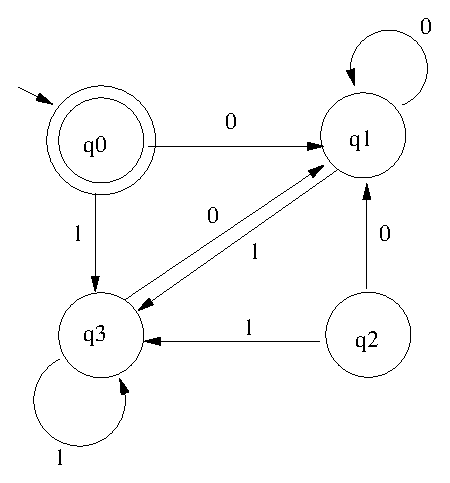
\includegraphics[width=10em]{fig}
%     \end{center}
%     \legend{Fonte: Os Autores}
%     \label{fig:ex1}
% \end{figure}

% % o `[h]' abaixo é um parâmetro opcional que sugere que o LaTeX coloque a
% % figura exatamente neste ponto do texto. Somente preocupe-se com esse tipo
% % de formatação quando o texto estiver completamente pronto (uma frase a mais
% % pode fazer o LaTeX mudar completamente de idéia sobre onde colocar as
% % figuras e tabelas)
% % \begin{figure}[h]
% \begin{figure}
%     \caption{Exemplo de figura desenhada com o environment \texttt{picture}.}
%     \begin{center}
%         \setlength{\unitlength}{.1em}
%         \begin{picture}(100,100)
%             \put(20,20){\circle{20}}
%             \put(20,20){\small\makebox(0,0){a}}
%             \put(80,80){\circle{20}}
%             \put(80,80){\small\makebox(0,0){b}}
%             \put(28,28){\vector(1,1){44}}
%         \end{picture}
%     \end{center}
%     \legend{Fonte: Os Autores}
%     \label{fig:ex2}
% \end{figure}